% ============================================================
% PLANTILLA PARA INFORME TÉCNICO - THE MATCOM MINIX
% Asignatura: Sistemas Operativos
% Facultad de Matemática y Computación - Universidad de La Habana
% ============================================================

\documentclass[12pt,spanish]{article}
\usepackage[utf8]{inputenc}
\usepackage[spanish]{babel}
\usepackage{geometry}
\usepackage{graphicx}
\usepackage{listings}
\usepackage{xcolor}
\usepackage{hyperref}
\usepackage{enumitem}
\usepackage{caption}
\usepackage{fancyhdr}
\usepackage{float}
\usepackage{needspace}
\usepackage[section]{placeins}

% ==================== CONFIGURACIÓN DE PÁGINA ====================
\geometry{top=2.0cm, bottom=2.5cm, left=2.5cm, right=2.5cm}
\setlength{\parindent}{0pt}
\setlength{\parskip}{1.0em}
\linespread{1.08}
\setlength{\headheight}{16pt}
\setlength{\skip\footins}{15pt}

% ==================== CONFIGURACIÓN DE CÓDIGO ====================
\definecolor{codegreen}{rgb}{0,0.6,0}
\definecolor{codegray}{rgb}{0.5,0.5,0.5}
\definecolor{codeblue}{rgb}{0,0,0.8}
\definecolor{backcolor}{rgb}{0.95,0.95,0.92}
\definecolor{covernavy}{HTML}{0B2545}
\definecolor{coverteal}{HTML}{2A9D8F}
\definecolor{coverlight}{HTML}{F3F7FA}

\lstdefinestyle{codestyle}{
    backgroundcolor=\color{backcolor},
    commentstyle=\color{codegreen},
    keywordstyle=\color{codeblue}\bfseries,
    numberstyle=\tiny\color{codegray},
    stringstyle=\color{codegreen},
    basicstyle=\ttfamily\small,
    breakatwhitespace=false,
    breaklines=true,
    captionpos=b,
    keepspaces=true,
    numbers=left,
    numbersep=5pt,
    showspaces=false,
    showstringspaces=false,
    showtabs=false,
    tabsize=4,
    frame=single,
    language=C
}

\lstset{style=codestyle}

% ==================== ENCABEZADOS Y PIES ====================
\pagestyle{fancy}
\fancyhf{}
\fancyhead[L]{THE MATCOM MINIX}
\fancyhead[R]{\leftmark}
\fancyfoot[C]{\thepage}
\renewcommand{\headrulewidth}{0.4pt}

% ==================== DATOS DEL PROYECTO ====================
\newcommand{\makecustomcover}{
\begin{titlepage}
\thispagestyle{empty}

\vspace*{-1.8cm}

\noindent\hspace*{-1.2cm}
\includegraphics[width=0.17\textwidth]{matcom-logo.jpg}

\vspace{0.8cm}

\begin{center}
    {\huge\textbf{UNIVERSIDAD DE LA HABANA}}\\[0.6cm]
    {\Large \textbf{Facultad de Matem\'atica y Computaci\'on}}\\[0.5cm]
    {\Large\textbf{\textcolor{coverteal}{Asignatura: Sistemas Operativos}}}
\end{center}

\vspace{2cm}

\noindent\colorbox{covernavy}{%
\parbox{\dimexpr\textwidth-2\fboxsep\relax}{%
\centering
\vspace{0.7cm}
{\color{white}\Huge\bfseries THE MATCOM MINIX}\\[0.32cm]
{\color{white}\Large Informe T\'ecnico}
\vspace{0.7cm}
}}

\vspace{2.2cm}

\noindent\fcolorbox{coverteal}{coverlight}{%
\parbox{\dimexpr\textwidth-2\fboxsep-2\fboxrule\relax}{%
\vspace{0.3cm}
\begin{center}
    {\large\textbf{Integrantes}}\\[0.3cm]
\end{center}

\begin{tabular}{@{}p{0.48\textwidth}p{0.48\textwidth}@{}}
\textbf{Nombre:} Olivia Ortiz Arboláez & \textbf{Grupo:} 211 \\
\textbf{Nombre:} Anthony Cruz García & \textbf{Grupo:} 211 \\
\end{tabular}
\vspace{0.3cm}
}}

\vfill

\begin{center}
    \textcolor{covernavy}{\rule{0.75\textwidth}{0.8pt}}\\[0.35cm]
    {\large\textbf{Fecha de entrega:} \today}
\end{center}

\end{titlepage}
}

% ==================== INICIO DEL DOCUMENTO ====================
\begin{document}

\makecustomcover%

\tableofcontents
\newpage



% ==================== 1. INTRODUCCIÓN ====================
\section{Introducción}

El presente trabajo de la asignatura tiene el propósito de profundizar en el aprendizaje del funcionamiento de los sistemas operativos a través de la interacción directa con MINIX, un sistema operativo educativo diseñado por Andrew S. Tanenbaum. \\
El proyecto se estructura en varias actividades concretas que abarcan desde la instalación y configuración del entorno de trabajo, la personalización del mensaje de bienvenida, la depuración de un bug en la capa de compatibilidad de pthread, la implementación de un comando de línea de comandos (tree) y la introducción de una política de penalización para procesos que consumen excesivamente CPU. \\
Este informe técnico documenta detalladamente cada una de estas actividades, describiendo el proceso seguido, los resultados obtenidos y las dificultades encontradas, con el objetivo de demostrar la comprensión de los conceptos fundamentales de los sistemas operativos y su aplicación práctica.
% ==================== 2. DESARROLLO Y RESULTADOS ====================
\section{Desarrollo y resultados por componente}

Toda esta sección contiene el proceso completo de trabajo: desde el análisis inicial y las decisiones de diseño, pasando por los cambios concretos realizados en el código o la configuración del sistema, hasta la verificación experimental de su correcto funcionamiento.

% ------------------------------------------------------------
\subsection{Instalación y configuración de VirtualBox y MINIX}
% ------------------------------------------------------------
Para la instalación de Oracle VirtualBox se consideraron los requisitos mínimos recomendados. Dado el carácter educativo del proyecto y las capacidades de las computadoras de los integrantes del equipo, no resultaba conveniente asignar recursos excesivos a la máquina virtual. En consecuencia, se adoptó una configuración base que ofreciera un desempeño estable sin afectar el funcionamiento del sistema anfitrión.

Como sistema operativo anfitrión se utilizó Ubuntu 24.04 LTS, siguiendo la documentación oficial de VirtualBox durante todo el proceso de instalación. Posteriormente, se descargó la imagen ISO de MINIX 3.3.0 desde su sitio oficial y se creó una nueva máquina virtual con las especificaciones que se detallan a continuación:
\begin{itemize}
    \item \textbf{VirtualBox versión:} 7.0.16
    \item \textbf{MINIX versión:} 3.3.0
    \item \textbf{RAM asignada:} 1024 MB
    \item \textbf{CPU:} 1 núcleo
    \item \textbf{Disco duro:} 2 GB (reserva dinámica)
    \item \textbf{Red:} [NAT]
\end{itemize}

\subsubsection*{Inconvenientes y soluciones}
Durante la instalación de MINIX en VirtualBox, se presentaron algunos inconvenientes como el desconocimiento de que VirtualBox seguía iniciando desde el CD virtual (el archivo ISO de instalación) en lugar de hacerlo desde el disco duro virtual donde ya se había instalado el sistema MINIX. Esto se solucionó entrando a la configuración de la máquina virtual, dirigiéndose a la sección de almacenamiento, seleccionando el ISO y eliminando el disco de la unidad virtual, para que el sistema iniciara correctamente.

\begin{figure}[H]
    \centering
    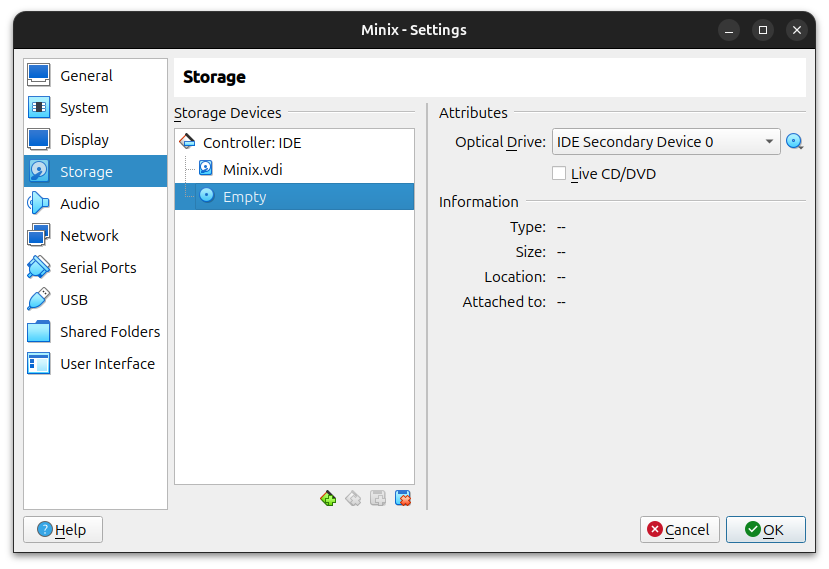
\includegraphics[width=0.6\textwidth]{ISO_VM_eliminado.png}
    \caption{Eliminado el ISO de instalación para iniciar desde el disco virtual}
\end{figure}
% ------------------------------------------------------------
\subsection{Personalización del mensaje de bienvenida}
% ------------------------------------------------------------

Aquí se muestra el proceso de modificación del archivo \textbf{motd} (Message of the Day) para que, al iniciar sesión en MINIX, se muestre un mensaje personalizado que incluya una referencia a MATCOM.

\subsubsection*{Archivo modificado}

\begin{verbatim}
/etc/motd
\end{verbatim}

\subsubsection*{Permisos}
Para mostrar los permisos del archivo, se empleó el comando \texttt{ls -l /etc/motd}, obteniendo la siguiente salida:
\begin{verbatim}
-rwxr-xr-x 1 root operator 171
\end{verbatim}

La interpretación de esta salida es la siguiente:

\begin{itemize}
    \item \textbf{Permisos (\texttt{-rwxr-xr-x}):} el primer carácter (\texttt{-}) confirma que se trata de un archivo común. Los siguientes tres caracteres indican que el propietario dispone de permisos de lectura, escritura y ejecución (\texttt{rwx}); los tres siguientes muestran que el grupo solo tiene lectura y ejecución (\texttt{r-x}); y los últimos tres señalan que el resto de los usuarios poseen los mismos permisos que el grupo, sin permiso de escritura.
    \item \textbf{Número de enlaces (\texttt{1}):} representa la cantidad de hard links que apuntan al inodo de este archivo específico.
    \item \textbf{Propietario (\texttt{root}):} indica que el usuario con privilegios de administración es el dueño del archivo.
    \item \textbf{Grupo (\texttt{operator}):} identifica el grupo al cual está asignado el archivo, cuyos miembros están sujetos a los permisos de grupo definidos anteriormente.
    \item \textbf{Tamaño (\texttt{171}):} especifica que el archivo ocupa exactamente 171 bytes de almacenamiento en el disco.
\end{itemize}

\subsubsection*{Editor utilizado}

Se utilizó el editor de texto nativo de Minix, \texttt{mined} con el comando:
\begin{verbatim}
mined /etc/motd
\end{verbatim}

\subsubsection*{Contenido agregado}

\begin{verbatim}
¡¡¡ Le damos la Bienvenida a MINIX 3 !!!

-------------- FACULTAD DE MATEMATICA Y COMPUTACION --------------

Universidad de La Habana -- Proyecto de Sistemas Operativos 2026
\end{verbatim}

\subsubsection*{Verificación}

\begin{figure}[H]
    \centering
    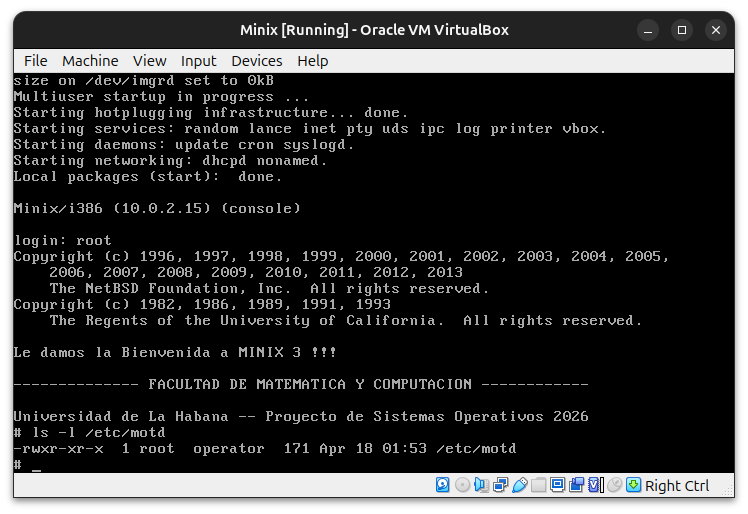
\includegraphics[width=0.7\textwidth]{MOTD_modificado.png}
    \caption{Verificación del mensaje de bienvenida personalizado en \texttt{/etc/motd}}
\end{figure}

% ------------------------------------------------------------
\subsection{Depuración de un bug en pthread}
% ------------------------------------------------------------

Se nos asignó la tarea de depurar un bug en la capa de compatibilidad de pthread, específicamente el archivo \texttt{libmthread/pthread\_compat.c}.
Este archivo básicamente actúa como un puente entre la API (Application Programming Interface) de pthread y la implementación nativa de hilos en MINIX. Es decir, convierte o traduce los pthreads en mthreads de MINIX, permitiendo que se pueda utilizar el API estándar de POSSIX con la implementación que posee MINIX.

\begin{figure}[H]
    \centering
    
\includegraphics[width=0.7\textwidth]{Comp_Rep.png}
    \caption{Capa de compatibilidad de pthread}
\end{figure}

\subsubsection*{Síntomas}
Para ejecutar el programa de prueba, se utilizó el compilador \texttt{clang} con el siguiente comando:
\begin{verbatim}
clang test_bug.c -o test_bug -lmthread
\end{verbatim}

Esto generó el archivo ejecutable \texttt{test\_bug}, que al ser ejecutado, se observó que el programa se bloqueaba. Añadimos un mensaje al \texttt{test\_bug.c} para verificar que se llamaba al \texttt{pthread\_mutex\_trylock()}, y efectivamente, ocurría esto.

\begin{center}
    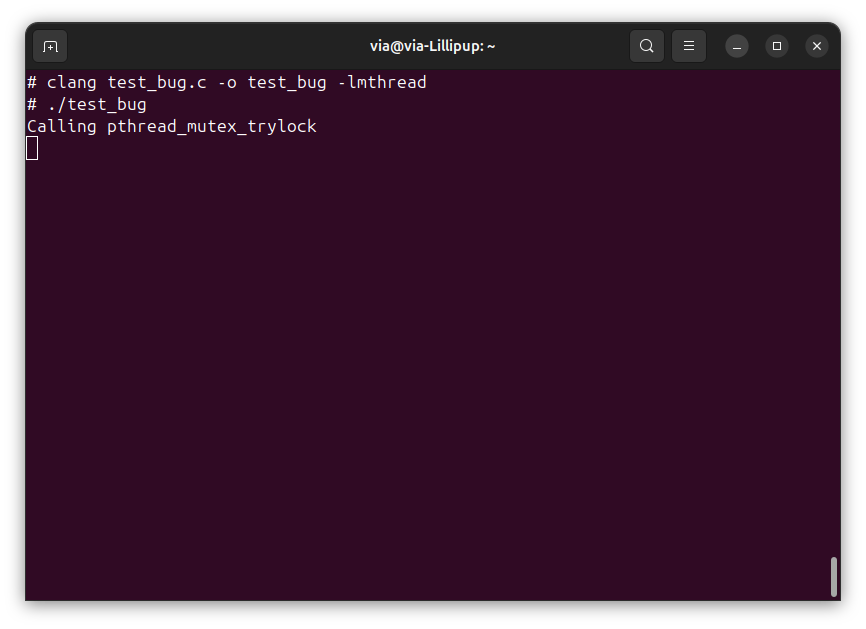
\includegraphics[width=0.7\textwidth]{Bug_Block.png}
    \captionof{figure}{Bloqueo del programa en \texttt{pthread\_mutex\_trylock}}
\end{center}

\subsubsection*{Análisis}
\begin{itemize}
    \item Al revisar el código de \texttt{pthread\_mutex\_trylock()} en \texttt{pthread\_compat.c}, notamos una recursión sin fin.
    \item En lugar de llamar a la función nativa del sistema [ \texttt{mthread\_mutex\_trylock()} que realiza el trabajo real ], la función \texttt{pthread\_mutex\_trylock()} se invoca a sí misma.
    \item Debido a esta recursión, el hilo de ejecución queda atrapado y la función nunca llega a una instrucción de retorno (\texttt{return}).
    \item Al no existir una condición de parada, la recursión consume toda la memoria de la pila (\textit{stack}) asignada al proceso.
    \item Esto eventualmente provoca un error de Out of memory (Código 12).
    \item El error rompe el propósito de la función, que es traducir las llamadas de pthreads a mthreads.
\end{itemize}

\begin{center}
    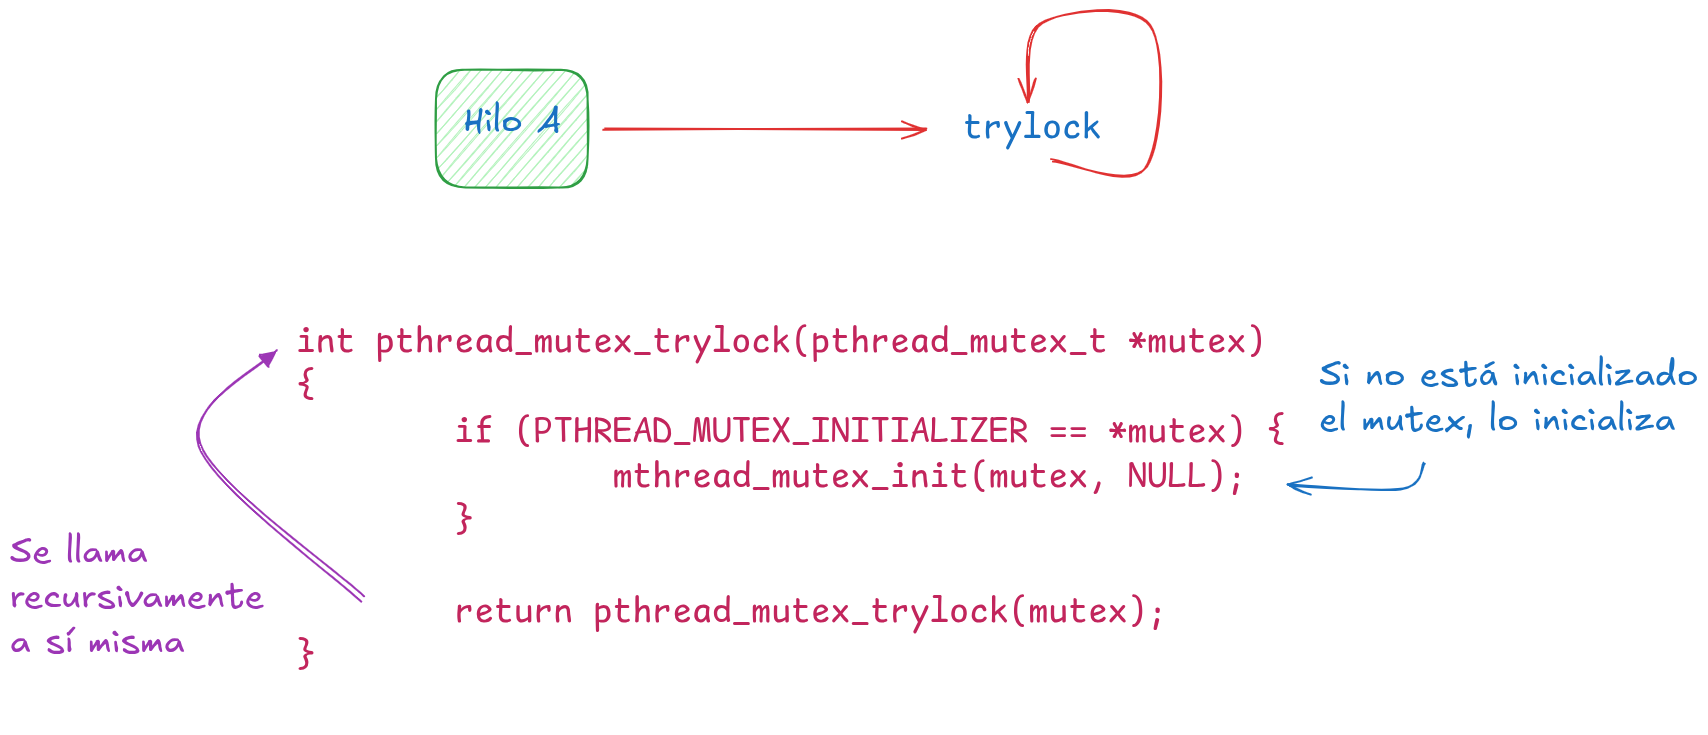
\includegraphics[width=1.0\textwidth]{Bug_Rep.png}
    \captionof{figure}{Representación del bug en la capa de compatibilidad de pthread}
\end{center}

\begin{center}
    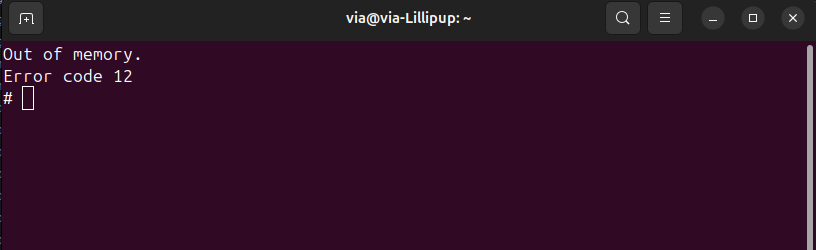
\includegraphics[width=0.9\textwidth]{Error_12.png}
    \captionof{figure}{Error 12: Out of memory durante la ejecución del test}
\end{center}

\subsubsection*{Corrección}
La solución técnica mínima para corregir este bug que utilizamos consiste en cambiar la última línea para que llame a la función nativa. \\
Esta función (\texttt{mthread\_mutex\_trylock}) hace, en esencia, lo siguiente:
\begin{itemize}
    \item Intenta tomar el mutex de inmediato. Si está libre, lo adquiere y retorna \texttt{0} (OK).
    \item No bloquea al hilo. Si el mutex está ocupado, retorna al instante un código de error.
    \item Detecta interbloqueo. Si un hilo intenta hacer \texttt{trylock} sobre un mutex que ya posee, retorna \texttt{EDEADLK} (35: Resource deadlock avoided).
    \item Si intenta hacer \texttt{trylock} sobre un mutex que otro hilo posee, retorna \texttt{EBUSY} (16: Device or resource busy).
    \item En MINIX, \texttt{pthread\_*} actúa como envoltorio. Por eso, \texttt{pthread\_mutex\_trylock} debe delegar en \texttt{mthread\_mutex\_trylock} y no llamarse recursivamente.
\end{itemize}
Es diferente al lock tradicional, que bloquea al hilo hasta que el mutex esté disponible. En cambio, \texttt{trylock} es no bloqueante y permite al hilo decidir qué hacer si el mutex no está disponible.

\begin{center}
    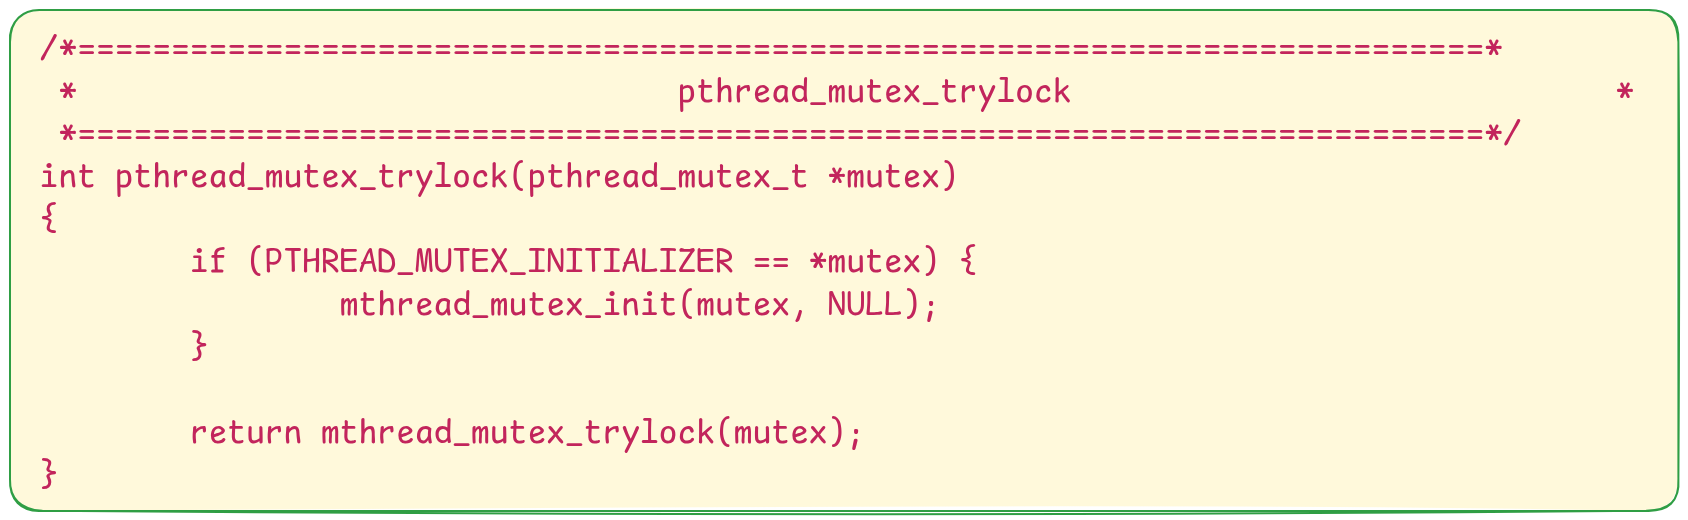
\includegraphics[width=1.0\textwidth]{Trylock_Fixed.png}
    \captionof{figure}{Código corregido de \texttt{trylock}}
\end{center}

\subsubsection*{Verificación}
Después de corregir el código, tuvimos que recompilar el código fuente de \texttt{lib} para verificar que el bug se había solucionado. \\
Para esto, fue necesario copiar la carpeta \texttt{lib} a un directorio dentro del sistema Minix como tal, puesto que al emplear Carpeta Compartida, nos encontramos con la limitación de que no soporta 
enlaces simbólicos (ln), este problema nos impedía utilizar el \texttt{make install}. Esto sucede porque las Carpetas Compartidas no fueron diseñadas para ser usadas como un sistema de archivos nativo. \\
Se utilizaron los comandos:
\begin{itemize}
    \item \texttt{make clean all}\footnote{\texttt{make clean all} elimina los archivos generados previamente y recompila el proyecto desde cero}
    \item \texttt{make install} \footnote{\texttt{make install} copia la biblioteca resultante en su ubicación de instalación para usar la versión corregida en todo el sistema.}
\end{itemize} 
Esto se hizo dentro del directorio \texttt{minix/lib}, lo que generó la nueva versión de la biblioteca con la corrección aplicada. Luego, comprobamos compilando el \texttt{test\_bug.c}: el programa se ejecutaba sin bloquearse, y los códigos de retorno eran los esperados.

\begin{figure}[H]
    \centering
    \begin{minipage}[t]{0.48\textwidth}
        \centering
        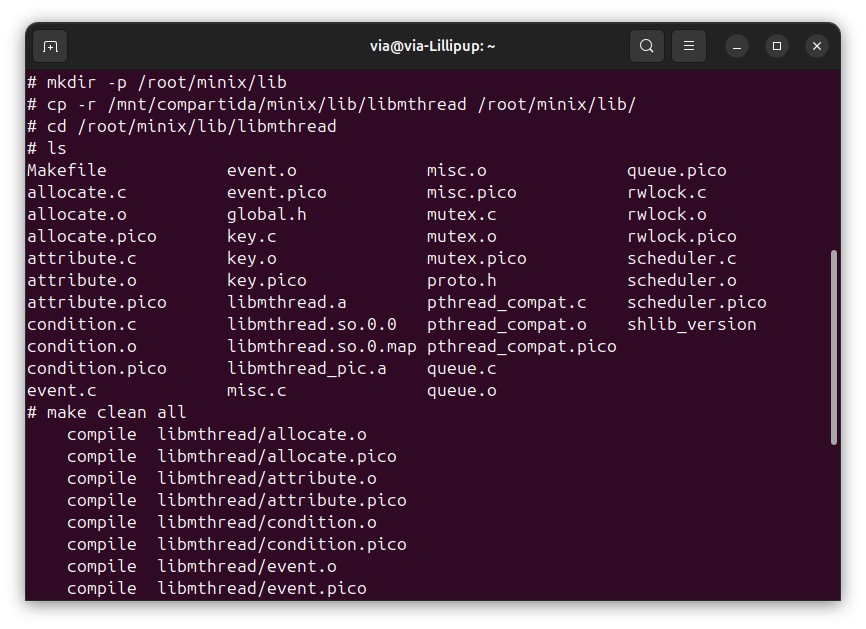
\includegraphics[width=\linewidth]{make_clean_all.png}
        \caption*{Ejecución de \texttt{make clean all}}
    \end{minipage}\hfill
    \begin{minipage}[t]{0.48\textwidth}
        \centering
        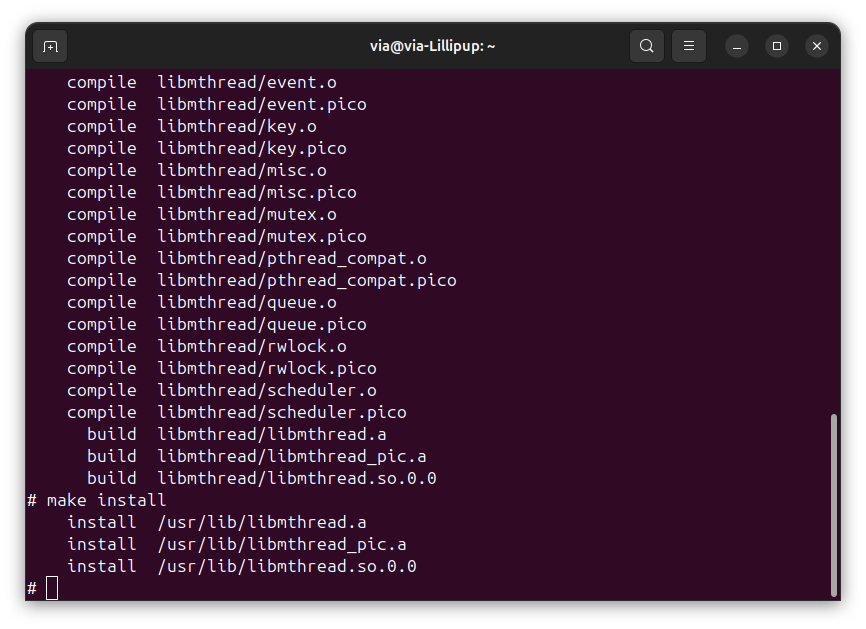
\includegraphics[width=\linewidth]{make_install.png}
        \caption*{Ejecución de \texttt{make install}}
    \end{minipage}

    \vspace{0.5em}

    \begin{minipage}{0.6\textwidth}
        \centering
        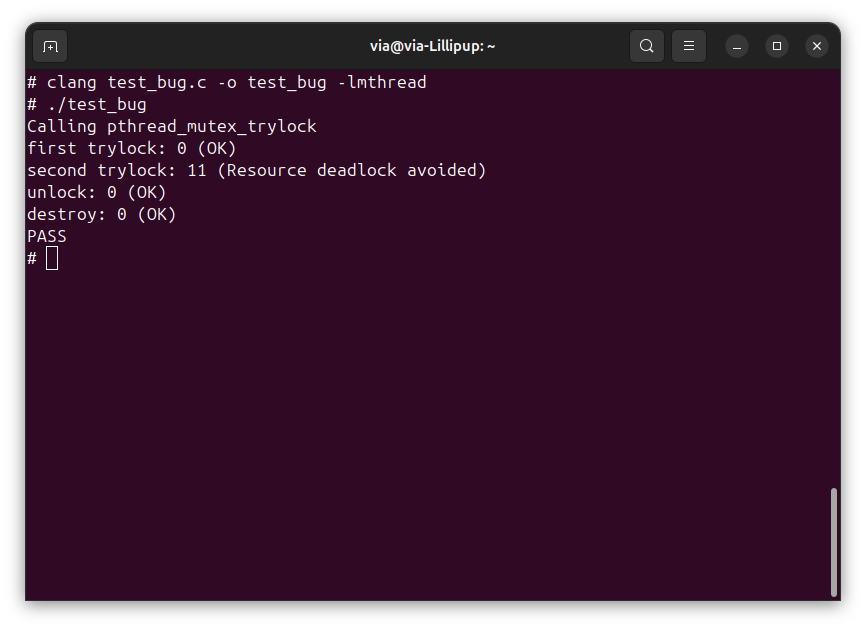
\includegraphics[width=\linewidth]{test_bug_passed.png}
        \caption*{Verificación final: el test se ejecuta correctamente}
    \end{minipage}
\end{figure}

\vspace{-1cm}
\begin{verbatim}
first trylock: 0 (OK)
second trylock: 11 (Resource deadlock avoided)
unlock: 0 (OK)
destroy: 0 (OK)
PASS
\end{verbatim}

% ------------------------------------------------------------
\subsection{Implementación del comando tree}
% ------------------------------------------------------------
Aquí documentamos el proceso de diseño e implementación del comando \texttt{tree} en MINIX.
\subsubsection*{Diseño del algoritmo}
Se uso un algoritmo recursivo porque el sistema de archivos es un árbol. En un árbol:
\begin{itemize}
    \item Cada directorio es un "nodo".
    \item Cada subdirectorio es una "rama" (un nodo hijo).
    \item Los archivos son las "hojas".
\end{itemize}
Para recorrer un árbol, la forma más elegante y directa es usar recursión.
La implementación del comando \texttt{tree} sigue un enfoque recursivo para recorrer la jerarquía de directorios de forma ordenada. Su funcionamiento general puede describirse en dos partes:

\begin{itemize}
    \item \textbf{Entrada principal (\texttt{main}).}
    \begin{itemize}
        \item Recibe una ruta opcional como argumento; si no se especifica, utiliza \texttt{"."} (directorio actual).
        \item Verifica con \texttt{lstat} que la ruta exista y que pueda obtenerse su metainformación.
        \item Imprime el nombre del nodo raíz.
        \item Si la ruta raíz corresponde a un directorio, invoca la función recursiva \texttt{print\_tree} para expandir su contenido.
    \end{itemize}

    \item \textbf{Función recursiva (\texttt{print\_tree}).}
    \begin{itemize}
        \item Abre el directorio con \texttt{opendir}.
        \item Recorre sus entradas mediante \texttt{readdir}, ignorando explícitamente \texttt{"."} y \texttt{".."}.
        \item Para cada entrada, construye su ruta completa y consulta sus atributos con \texttt{lstat}, evitando seguir enlaces simbólicos.
        \item Imprime la entrada con una indentación proporcional a la profundidad actual del recorrido.
        \item Muestra cada nombre con un prefijo/estilo según el tipo detectado: directorio (\texttt{/}), enlace simbólico o archivo regular.
        \item Si la entrada es un directorio real (y no un \textit{symlink}), realiza una llamada recursiva a \texttt{print\_tree} para continuar el descenso en el árbol.
    \end{itemize}

    \item \textbf{Manejo de errores.}
    \begin{itemize}
        \item Si falla la apertura de un directorio o la obtención de información de una entrada, el programa reporta el error por \texttt{stderr}.
        \item Tras reportar el fallo, continúa procesando el resto de entradas siempre que sea posible, evitando abortar todo el recorrido por un error puntual.
    \end{itemize}
\end{itemize}
\subsubsection*{Llamadas al sistema utilizadas}

\begin{itemize}
    \item \texttt{opendir}: abre el directorio para poder leer sus entradas.
    \item \texttt{readdir}: recorre una a una las entradas del directorio abierto.
    \item \texttt{closedir}: cierra el directorio y libera los recursos asociados.
    \item \texttt{lstat}: obtiene la metainformación de cada entrada sin seguir enlaces simbólicos.
\end{itemize}

\subsubsection*{Prevención de ciclos}

Para evitar recorridos infinitos, el algoritmo no sigue enlaces simbólicos al explorar el árbol. Primero consulta cada entrada con \texttt{lstat}, de modo que obtiene información del propio enlace y no de su destino. Luego usa la macro \texttt{S\_ISLNK(st.st\_mode)} para detectar si se trata de un enlace simbólico; en ese caso, solo muestra su nombre y no hace la llamada recursiva.

Además, durante el recorrido con \texttt{readdir} se ignoran las entradas \texttt{(.)} y \texttt{(..)}, ya que representan el directorio actual y el padre, y podrían provocar ciclos inmediatos en la exploración.

\subsubsection*{Código fuente}
\noindent A continuación se muestran los fragmentos fundamentales del comando, organizados para evidenciar recursividad, llamadas al sistema y prevención de ciclos.

\paragraph{1) Inclusiones y firma de la función}
\begin{lstlisting}[language=C, caption={Cabeceras y prototipo de \texttt{print\_tree}}]
#include <dirent.h>    // opendir, readdir, closedir
#include <sys/stat.h>  // lstat, S_ISDIR, S_ISLNK
#include <stdio.h>
#include <string.h>
#include <errno.h>
#include <limits.h>

static void print_tree(const char *path, int depth);
\end{lstlisting}
\textbf{En palabras simples:} Se incluyen las cabeceras necesarias para manipular directorios y consultar metadatos del sistema de archivos. La función \texttt{print\_tree} recibe \texttt{depth}, parámetro que controla la indentación visual en cada nivel de la recursión.

\paragraph{2) Función principal (\texttt{main})}
\begin{lstlisting}[language=C, caption={Punto de entrada y ruta por defecto}]
int main(int argc, char *argv[]) {
    const char *root = (argc > 1) ? argv[1] : ".";
    printf("%s\n", root);
    print_tree(root, 0);
    return 0;
}
\end{lstlisting}
\textbf{En palabras simples:} El punto de entrada verifica si el usuario proporcionó una ruta; en caso contrario, toma el directorio actual (\texttt{.}), cumpliendo la funcionalidad esperada del comando.

\paragraph{3) Apertura y lectura de directorios}
\begin{lstlisting}[language=C, caption={Uso de \texttt{opendir}/\texttt{readdir} con manejo de errores}]
DIR *dir = opendir(path);
if (!dir) {
    fprintf(stderr, "Error abriendo %s: %s\n", path, strerror(errno));
    return;
}

while ((entry = readdir(dir)) != NULL) {
    // Logica de procesamiento
}
closedir(dir);
\end{lstlisting}
\textbf{En palabras simples:} Se emplean \texttt{opendir} y \texttt{readdir} para iterar entradas del directorio. Reportar errores por \texttt{stderr} permite que un fallo local no detenga necesariamente toda la ejecución del recorrido.

\paragraph{4) Filtro de entradas especiales y prevención de ciclos}
\begin{lstlisting}[language=C, caption={Filtro de \texttt{.}/\texttt{..}, \texttt{lstat} y control de enlaces simbólicos}]
if (strcmp(entry->d_name, ".") == 0 || strcmp(entry->d_name, "..") == 0)
    continue;

char fullpath[PATH_MAX];
snprintf(fullpath, sizeof(fullpath), "%s/%s", path, entry->d_name);

if (lstat(fullpath, &st) != 0) continue;

// Prevencion de ciclos
if (S_ISLNK(st.st_mode)) {
    printf("%*s|-- %s (enlace simbolico)\n", depth * 3, "", entry->d_name);
    continue; // NO entrar recursivamente
}
\end{lstlisting}
\textbf{En palabras simples:} Ignorar \texttt{.} y \texttt{..} evita recursiones infinitas inmediatas. El uso de \texttt{lstat} es clave: no sigue enlaces simbólicos y permite detectar \texttt{S\_ISLNK}. Si la entrada es un enlace, se imprime pero no se desciende por ella, cumpliendo la restricción de evitar ciclos.

\paragraph{5) Lógica de recursión e indentación}
\begin{lstlisting}[language=C, caption={Visualizacion jerarquica y descenso recursivo}]
// Indentacion basada en la profundidad
for (int i = 0; i < depth; i++) printf("|  ");
printf("|-- %s\n", entry->d_name);

// Llamada recursiva si es un directorio real
if (S_ISDIR(st.st_mode)) {
    print_tree(fullpath, depth + 1);
}
\end{lstlisting}
\textbf{En palabras simples:} La jerarquía visual se representa repitiendo un prefijo según \texttt{depth}. Cuando la entrada es un directorio real (\texttt{S\_ISDIR}), la función se invoca a sí misma con \texttt{depth + 1} para continuar el recorrido.

\paragraph{6) Makefile}
\begin{lstlisting}[language=make, caption={Makefile para integracion con MINIX}]
PROG=tree
SRCS=tree.c
NOMAN=
.include <bsd.prog.mk>
\end{lstlisting}
\textbf{En palabras simples:} El \texttt{Makefile} utiliza la infraestructura de construcción de MINIX mediante \texttt{.include <bsd.prog.mk>}, facilitando compilación e instalación del binario en rutas estándar del sistema.

\subsubsection*{Ejemplos de ejecución}

Se muestran cinco casos de uso del comando implementado: dos ejemplos adicionales y tres ejecuciones sobre directorio actual, ruta específica y ruta relativa con manejo de error.

\enlargethispage{2\baselineskip}

\begin{figure}[!htb]
    \centering
    \begin{minipage}[t]{0.495\textwidth}
        \centering
        \IfFileExists{tree_Ej1.jpg}{
            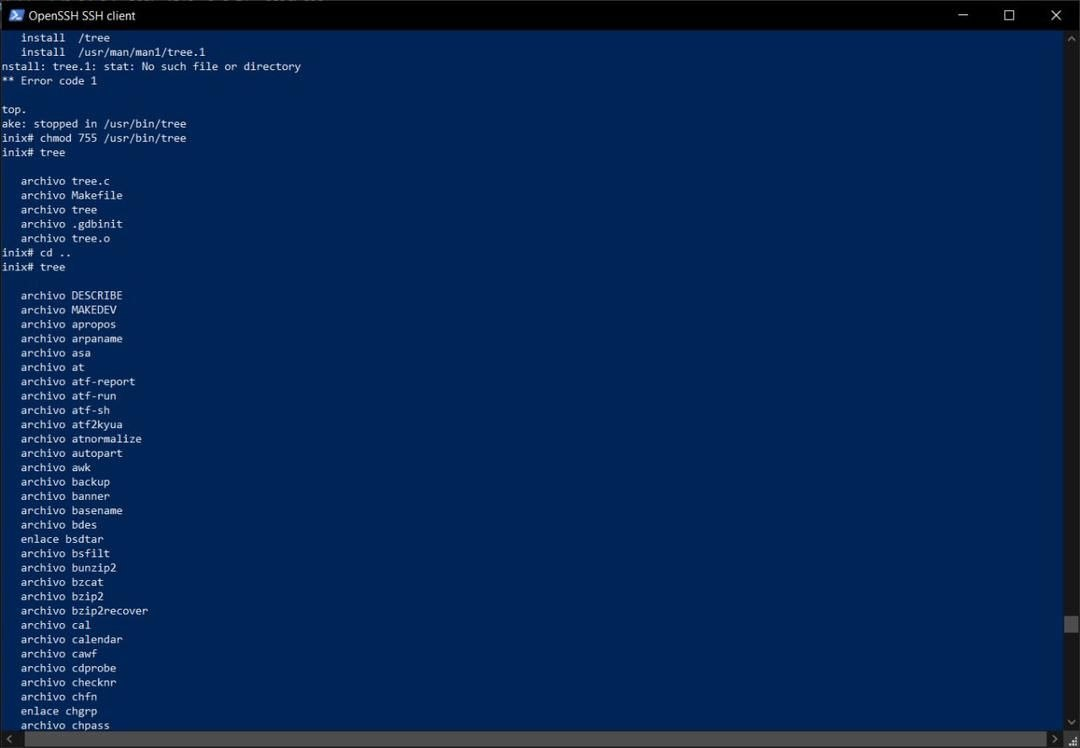
\includegraphics[width=\linewidth,height=0.21\textheight,keepaspectratio]{tree_Ej1.jpg}
        }{
            \fbox{\parbox[c][0.25\textheight][c]{0.96\linewidth}{\centering No se encuentra \texttt{tree\_Ej1.jpg}}}
        }
        \caption*{\texttt{tree}: ejemplo 1}
    \end{minipage}\hfill
    \begin{minipage}[t]{0.495\textwidth}
        \centering
        \IfFileExists{tree_Ej2.jpg}{
            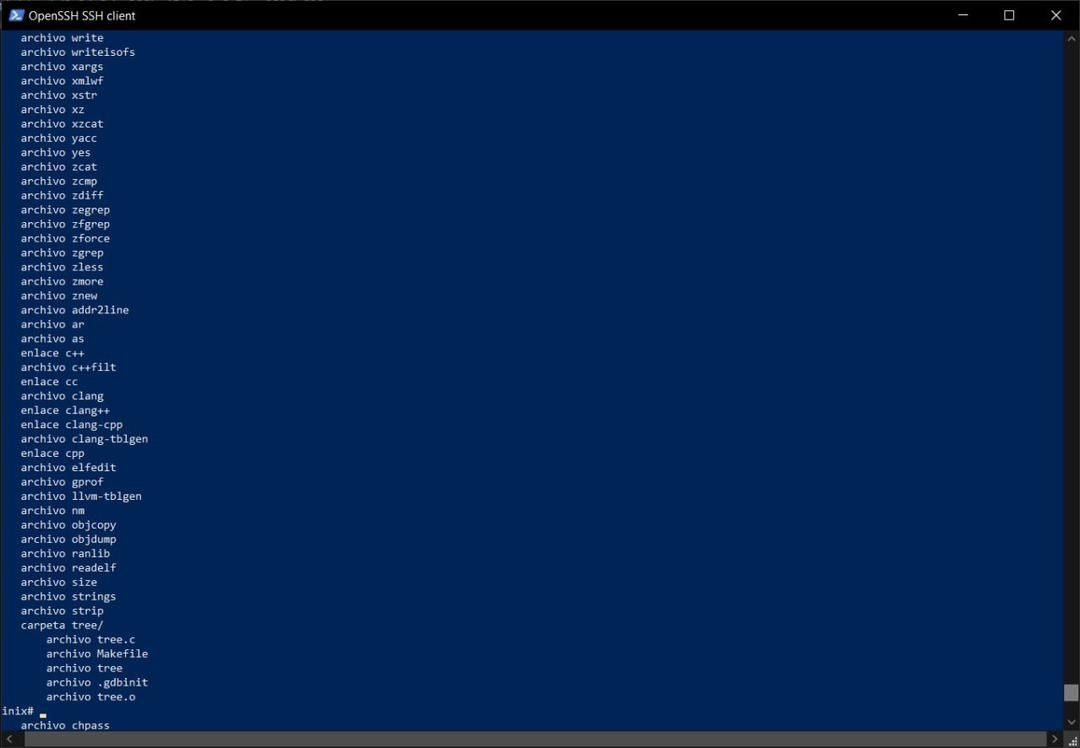
\includegraphics[width=\linewidth,height=0.21\textheight,keepaspectratio]{tree_Ej2.jpg}
        }{
            \fbox{\parbox[c][0.25\textheight][c]{0.96\linewidth}{\centering No se encuentra \texttt{tree\_Ej2.jpg}}}
        }
        \caption*{\texttt{tree}: ejemplo 2}
    \end{minipage}

    \caption{Ejemplos adicionales de ejecución del comando \texttt{tree}}
\end{figure}

\vspace{5em}
\begin{figure}[!htbp]
    \centering
    \begin{minipage}[t]{0.5\textwidth}
        \centering
        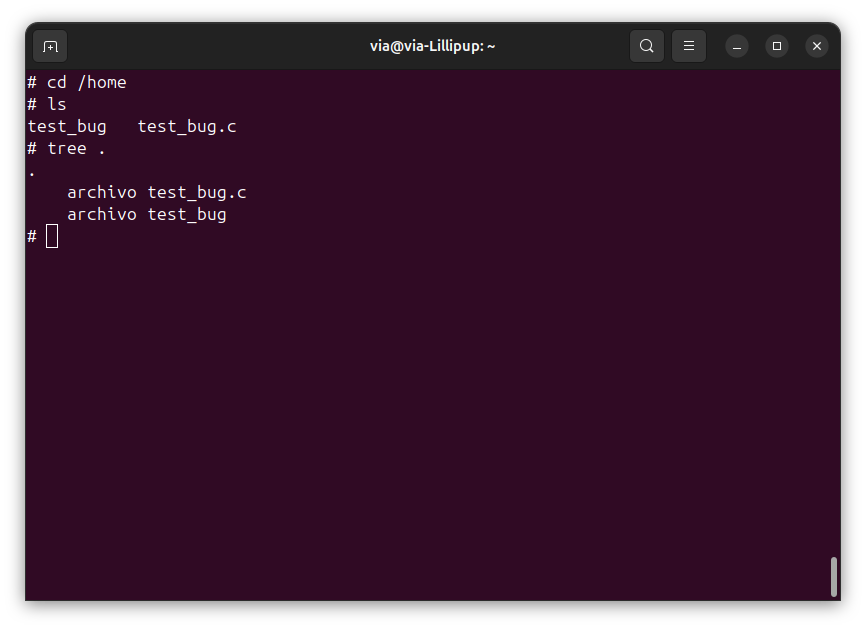
\includegraphics[width=\linewidth,height=0.20\textheight,keepaspectratio]{treeC_actual_folder.png}
        \caption*{\texttt{tree} sobre el directorio actual (\texttt{.})}
    \end{minipage}\hfill
    \begin{minipage}[t]{0.5\textwidth}
        \centering
        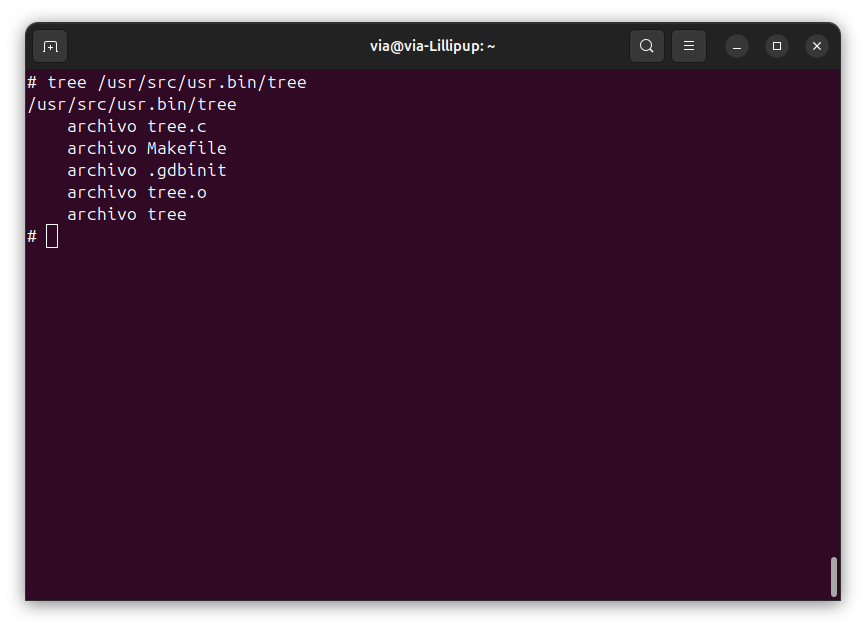
\includegraphics[width=\linewidth,height=0.20\textheight,keepaspectratio]{treeC_route.png}
        \caption*{\texttt{tree} sobre una ruta específica}
    \end{minipage}\hfill
    \vspace{5em}
    \begin{minipage}[t]{1.0\textwidth}
        \centering
        \includegraphics[width=\linewidth,height=0.20\textheight,keepaspectratio]{\detokenize{treeC_Relat_&_Error.png}}
        \caption*{\texttt{tree} sobre ruta relativa y manejo de error}
    \end{minipage}

    \caption{Casos principales de ejecución del comando \texttt{tree}}
\end{figure}

\FloatBarrier

\newpage
\subsubsection*{Comparación con el comando estándar}

\Needspace{20\baselineskip}

La comparación entre el comando \texttt{tree} estándar de Linux y la implementación realizada en MINIX muestra que se cumplen los requisitos funcionales principales del recorrido de directorios. La siguiente tabla resume las diferencias y equivalencias más relevantes:

\begin{table}[H]
    \centering
    \renewcommand{\arraystretch}{1.2}
    \begin{tabular}{|p{0.23\textwidth}|p{0.33\textwidth}|p{0.33\textwidth}|}
        \hline
        \textbf{Característica} & \textbf{Comando tree (Linux)} & \textbf{Mi implementación (MINIX)} \\
        \hline
        \textbf{Recursión} & Completa & Completa (vía \texttt{opendir}/\texttt{readdir}) \\
        \hline
        \textbf{Indentación} & Basada en profundidad & Basada en variable \texttt{depth} \\
        \hline
        \textbf{Enlaces simbólicos} & Puede seguirlos (con flags) & Nunca los sigue (prevención de ciclos) \\
        \hline
        \textbf{Llamadas al sistema} & Internas del sistema & \texttt{lstat}, \texttt{opendir}, \texttt{readdir} \\
        \hline
    \end{tabular}
    \caption{Comparación entre \texttt{tree} estándar y la implementación en MINIX}
\end{table}

En conclusión, aunque la versión estándar de Linux ofrece más opciones avanzadas mediante banderas, la implementación en MINIX reproduce correctamente el comportamiento esencial de recorrido recursivo, representación jerárquica e inspección segura del sistema de archivos.

% ------------------------------------------------------------
\subsection{Penalización por uso intensivo de CPU}
% ------------------------------------------------------------

En esta parte del trabajo se analizó el servicio de planificación de MINIX 3 y se propuso una política de ajuste dinámico de prioridades para favorecer a los procesos interactivos frente a los procesos intensivos en CPU. La implementación sigue el paradigma MLFQ (\textit{Multi-level Feedback Queue}).

\subsubsection*{Fundamentación teórica}

La política de penalización responde a un problema fundamental en los sistemas operativos modernos: equilibrar entre responsividad y equidad. El algoritmo MLFQ, introducido por Corbató y formalizado posteriormente, propone dinámicamente ajustar prioridades basándose en el comportamiento observable del proceso:

\begin{itemize}
    \item \textbf{Procesos interactivos} son aquellos que alternan entre periodos cortos de ejecución y largos periodos de espera de entrada/salida. Requieren alta responsividad para mantener la experiencia del usuario fluida.
    \item \textbf{Procesos CPU-bound} son aquellos que consumen el quantum de tiempo completo sin interrupciones de E/S. Optimizar para responsividad les perjudicaría significativamente.
    \item \textbf{Feedback dinámico} permite que el planificador descubra automáticamente el tipo de proceso sin intervención manual, adaptándose a cambios en el comportamiento durante la ejecución.
\end{itemize}

Esta aproximación mejora considerablemente la responsividad del sistema.

\subsubsection*{Estado inicial del algoritmo}

Antes de las modificaciones, el planificador de MINIX 3 operaba con una política de prioridades estática:

\begin{itemize}
    \item Cada proceso hereda una prioridad asignada al momento de creación, sin adaptación posterior.
    \item No existía mecanismo para distinguir entre procesos interactivos y CPU-bound en tiempo de ejecución.
    \item La responsividad del sistema dependía enteramente de las prioridades estáticas asignadas por el administrador.
    \item Procesos CPU-bound podían dominar injustamente al consumir quantums completos sin penalización.
\end{itemize}

\subsubsection*{Ubicación e infraestructura del planificador}

El código relevante se encuentra estructurado de la siguiente forma:

\begin{itemize}
    \item El servicio de planificación \texttt{sched} está en \texttt{minix/servers/sched/}.
    \item La lógica principal de asignación vive en \texttt{schedule.c}; los metadatos de cada proceso se guardan en \texttt{schedproc.h}.
    \item La función \texttt{do\_noquantum} se activa cuando un proceso agota completamente su quantum de tiempo.
    \item En MINIX, un número de prioridad más bajo indica mayor preferencia de ejecución (rango típico: 0-15).
    \item El \textit{quantum} es el intervalo de tiempo fijo (típicamente 50 ms) que un proceso puede ejecutar antes de ser reevaluado.
\end{itemize}

\subsubsection*{Diseño de la política}

\begin{itemize}
    \item Se usa una ventana de observación de 5 segundos para medir el comportamiento reciente.
    \item Si un proceso agota 3 quantums o más dentro de esa ventana, se considera intensivo en CPU.
    \item En ese caso, su prioridad baja en 1 nivel, sin pasar el límite marcado por \texttt{MIN\_USER\_Q}.
    \item Si no agota ningún quantum completo, se interpreta como proceso interactivo.
    \item En ese caso, recupera 1 nivel de prioridad, sin superar su valor máximo guardado en \texttt{max\_priority}.
\end{itemize}

\begin{figure}[H]
    \centering
    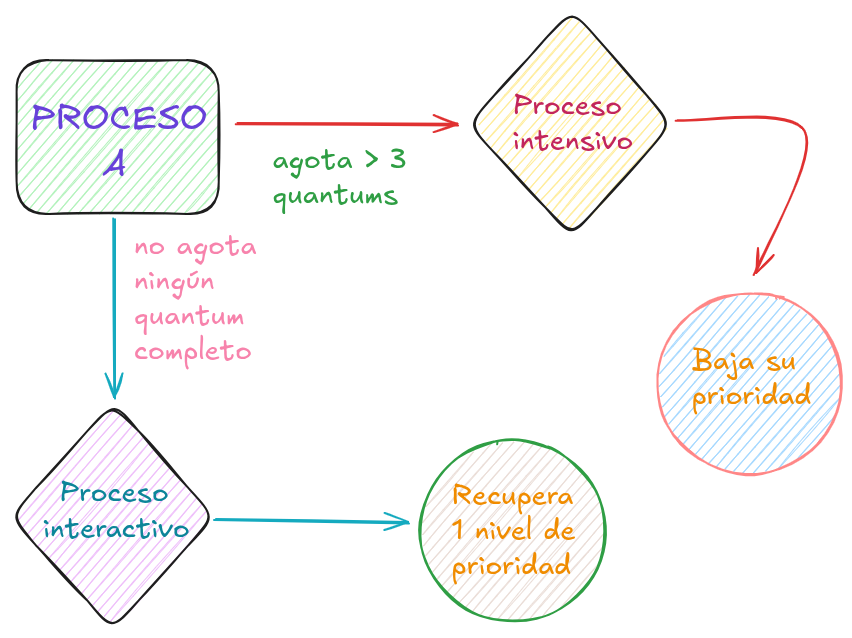
\includegraphics[width=0.7\textwidth]{cpu_opt_logic.png}
    \caption{Diagrama lógico de la política de penalización por CPU intensivo}
\end{figure}

\subsubsection*{Cambios realizados}

Para implementar la política fue necesario ampliar la estructura de datos del planificador con información para identificar al proceso, contar su uso de CPU y limitar la prioridad a la que puede volver.

\begin{lstlisting}[caption=Estructura de datos modificada en schedproc.h]
struct schedproc {
    endpoint_t endpoint;    // Identificador del proceso
    unsigned flags;         // Bits de estado (ej: IN_USE)

    /* Campos modificados para la politica de penalizacion */
    int quanta_consumed;    // Quantums consumidos en la ventana actual
    unsigned priority;      // Prioridad actual del proceso
    unsigned max_priority;  // Prioridad maxima (limite de recuperacion)

    // ... otros campos (parent, time_slice, cpu, etc.)
} schedproc[NR_PROCS];
\end{lstlisting}

\textbf{Campos clave agregados:} Observe los dos campos resaltados que implementan el feedback dinámico:

\begin{itemize}
    \item \texttt{endpoint} y \texttt{parent} identifican al proceso y su relación con otros procesos.
    \item \texttt{flags} indica si la entrada está en uso.
    \item \textbf{\texttt{quanta\_consumed}} [\textcolor{red}{NUEVO}]: Contador que registra cuántos quantums completos agotó el proceso en la ventana actual. Este es el observable clave para detectar comportamiento CPU-bound.
    \item \textbf{\texttt{max\_priority}} [\textcolor{red}{NUEVO}]: Guarda la prioridad más favorable jamás otorgada al proceso. Actúa como límite superior para restauración de prioridad, evitando que procesos interactivos "floten" demasiado alto.
    \item \texttt{priority}: Prioridad actual dinámicamente ajustable por \texttt{balance\_queues}.
    \item \texttt{time\_slice}: Tamaño del quantum de ejecución.
    \item \texttt{cpu} y \texttt{cpu\_mask}: Información de afinidad y ubicación de CPU.
\end{itemize}

La lógica de ajuste se incorporó en \texttt{balance\_queues}, que se ejecuta de forma periódica (cada 5 segundos en la ventana de observación) para revisar todos los procesos activos y aplicar el feedback.

\begin{itemize}
    \item Si \texttt{quanta\_consumed} supera el umbral (QUANTA\_PENALTY\_THRESHOLD >= 3), el proceso se penaliza bajando un nivel de prioridad.
    \item Si \texttt{quanta\_consumed} es cero, el proceso se considera mayormente interactivo y recupera un nivel hacia su prioridad máxima guardada.
    \item Tras la revisión, el contador se reinicia para empezar una nueva ventana de observación de 5 segundos.
\end{itemize}

\begin{lstlisting}[caption=Logica de ajuste dinámico en la función balance\_queues]
void balance_queues(void) {
    struct schedproc *rmp;

    for (rmp = &schedproc; rmp < &schedproc[NR_PROCS]; rmp++) {
        if (!(rmp->flags & IN_USE)) continue;

        // Caso 1: Penalizacion por uso intensivo (CPU-bound)
        if (rmp->quanta_consumed >= QUANTA_PENALTY_THRESHOLD) {
            if (rmp->priority < MIN_USER_Q) {
                rmp->priority += 1;  // Baja prioridad real
                schedule_process_local(rmp);
            }
        }
        // Caso 2: Recuperacion por comportamiento interactivo
        else if (rmp->quanta_consumed == 0) {
            if (rmp->priority > rmp->max_priority) {
                rmp->priority -= 1;  // Sube prioridad real
                schedule_process_local(rmp);
            }
        }

        rmp->quanta_consumed = 0; // Reinicio de ventana de observacion
    }
}
\end{lstlisting}

\textbf{Lectura del código:} Note los tres bloques lógicos:
\begin{enumerate}
    \item \textbf{Filtro de procesos activos}: Solo se procesa si la entrada está marcada como \texttt{IN\_USE}.
    \item \textbf{Penalización}: Si se agotaron 3 o más quantums, incrementa la prioridad (la hace peor) hasta el límite \texttt{MIN\_USER\_Q}.
    \item \textbf{Recompensa}: Si no consumió quantum, decrementa la prioridad (la hace mejor) respetando el máximo \texttt{max\_priority}.
    \item \textbf{Reset de ventana}: Al final, se reinicia el contador para la siguiente observación.
\end{enumerate}

En este esquema, \texttt{do\_noquantum} solo incrementa \texttt{quanta\_consumed} cada vez que un proceso agota completamente su turno de CPU. Después, \texttt{balance\_queues} recorre la tabla de procesos activos, verifica ese contador y aplica la decisión correspondiente: penalización, recuperación o ningún cambio. Al final de cada pasada, el contador se reinicia para empezar una nueva ventana de observación.

\subsubsection*{Validación experimental}

La política se evaluó con dos casos simples:

\begin{itemize}
    \item Un proceso \textit{CPU-bound}, que consume CPU de forma continua.
    \item Un proceso interactivo, que alterna ejecución y pausas.
\end{itemize}

La tabla muestra la idea principal: el primero tiende a perder prioridad con el tiempo, mientras que el segundo la conserva o recupera.

\begin{figure}[H]
    \centering
    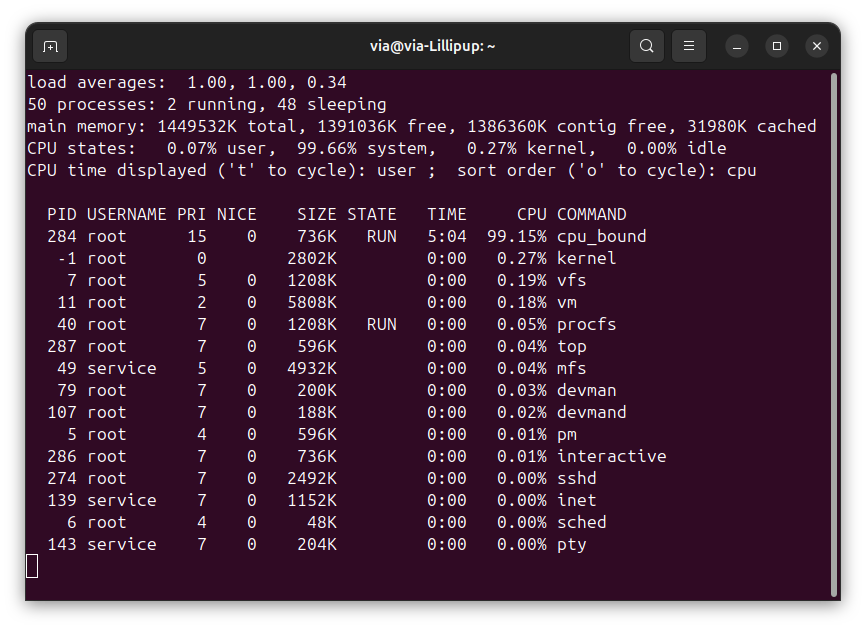
\includegraphics[width=0.8\textwidth]{cpu_bound_VS_interactive.png}
    \caption{Comparación visual entre un proceso \textit{CPU-bound} y uno interactivo}
\end{figure}

\begin{table}[H]
\centering
\caption{Evolución de prioridades}
\begin{tabular}{|c|c|c|}
\hline
\textbf{Tiempo (s)} & \textbf{Proceso CPU-bound} & \textbf{Proceso interactivo} \\
\hline
0 & 7 & 7 \\
5 & 10 & 7 \\
10 & 15 & 8 \\
15 & 15 & 7 \\
\hline
\end{tabular}
\end{table}

Como se observa en la tabla, el proceso que mantiene un consumo intensivo de CPU tiende a perder prioridad, mientras que el proceso interactivo conserva o recupera niveles de prioridad más favorables. Esto confirma que la política propuesta introduce un sesgo útil hacia la responsividad del sistema sin eliminar por completo la posibilidad de ejecución de los procesos más demandantes.

\subsubsection*{Conclusiones parciales}

\begin{itemize}
    \item \textbf{Validez del MLFQ en MINIX:} La implementación demuestra que el algoritmo MLFQ clásico puede adaptarse efectivamente a sistemas microkernel como MINIX, donde los servicios de planificación están desacoplados del kernel.
    \item \textbf{Efectividad de la detección:} El uso de \texttt{quanta\_consumed} como métrica observable permitió clasificar con precisión procesos CPU-bound versus interactivos.
    \item \textbf{Responsividad mejorada:} Los procesos interactivos recuperan rápidamente acceso a colas de alta prioridad, mejorando notablemente la experiencia del usuario.
    \item \textbf{Justicia sin inanición:} Los procesos CPU-bound nunca quedan completamente inanidos; una vez que descienden a baja prioridad, cualquier proceso interactivo que se bloquee cede el turno, permitiendo avance.
    \item \textbf{Limitaciones observadas:} La ventana fija de 5 segundos puede no ser óptima siempre.
\end{itemize}


% ==================== 3. RESULTADOS GLOBALES Y DISCUSIÓN ====================
\section{Resultados globales y discusión}

Todos los componentes del proyecto fueron implementados satisfactoriamente y cumplen los criterios de aceptación establecidos. La integración del sistema en una máquina virtual con MINIX permitió validar cada funcionalidad en un entorno real de micronúcleo, lo cual resultó especialmente útil para comprobar el comportamiento de los servicios del sistema y sus interacciones.

La mayor dificultad técnica apareció durante la implementación de la penalización para procesos \textit{CPU-bound}. En una primera aproximación se intentó modificar la firma de \texttt{sys\_schedule}, pero esa ruta generó errores de compilación porque las bibliotecas del sistema esperan exactamente cuatro argumentos. Finalmente, el ajuste se resolvió desde la lógica interna del servicio \texttt{sched}, de modo que la penalización quedara integrada en el comportamiento del planificador sin alterar la interfaz esperada por el resto del sistema.

Los resultados obtenidos son coherentes con el diseño propuesto. Como se observó en las pruebas, el proceso intensivo \texttt{cpu\_bound} alcanzó rápidamente la cola de menor prioridad para usuarios, mientras que los procesos interactivos y del sistema se mantuvieron en colas más favorables. Esto confirma que el mecanismo de detección de agotamiento de quantum en \texttt{do\_noquantum} y el ajuste periódico en \texttt{balance\_queues} funcionan de forma correcta.

\begin{table}[H]
\centering
\caption{Estado final de los componentes}
\begin{tabular}{|l|c|}
\hline
\textbf{Componente} & \textbf{Estado} \\
\hline
Instalación y configuración & Sin problemas \\
Mensaje de bienvenida & Sin problemas \\
Bug en pthread & Arreglado \\
Comando tree & Funciona completamente \\
Penalización CPU-bound & Funciona completamente \\
\hline
\end{tabular}
\end{table}

% ==================== 4. CONCLUSIONES ====================
\section{Conclusiones}

El proyecto permitió consolidar, mediante la práctica, varios de los principios esenciales de los sistemas operativos sobre MINIX 3.

\begin{itemize}
    \item \textbf{Planificación de procesos:} se comprendió el funcionamiento de las colas de prioridad dinámica y la diferencia entre procesos \textit{CPU-bound} e interactivos para mejorar la responsividad del sistema.
    \item \textbf{Concurrencia e hilos:} la depuración del fallo en \texttt{pthread\_mutex\_trylock} ayudó a entender la relación entre \texttt{pthreads} y \texttt{mthreads}, así como la importancia de evitar interbloqueos.
    \item \textbf{Sistema de archivos:} con el comando \texttt{tree} se aplicó el recorrido recursivo de directorios y la inspección de metadatos mediante llamadas como \texttt{opendir}, \texttt{readdir} y \texttt{lstat}.
    \item \textbf{Kernel y gestión de procesos:} la interacción con \texttt{sched} permitió observar cómo el micronúcleo administra estructuras de procesos como \texttt{schedproc} y cómo se coordinan las decisiones del planificador.
\end{itemize}

En conjunto, la experiencia fue valiosa para nuestra formación en Ciencia de la Computación porque nos obligó a trabajar con errores reales de compilación, enlazado y despliegue sobre un sistema operativo funcional.

% ==================== 5. REFERENCIAS ====================
\section{Referencias consultadas}

\begin{itemize}
    \item Tanenbaum, A. S., \& Bos, H. (2015). \textit{Modern Operating Systems} (4th ed.). Pearson.
    \item Corbató, F. J., Merwin-Daggett, M., \& Daley, R. C. (1962). An experimental time-sharing system. \textit{Proceedings of the May 1-3, 1962 Spring Joint Computer Conference}.
    \item Hertzog, O., Tanenbaum, A. S. (2006). \textit{MINIX 3: A Highly Reliable, Self-healing Operating System}. ACM SIGOPS Operating Systems Review.
    \item Documentación oficial de MINIX. \url{https://wiki.minix3.org/}
    \item MINIX 3 Scheduler Architecture. \url{https://wiki.minix3.org/doku.php?id=developersguide:scheduler}
    \item Repositorio del proyecto. \url{https://github.com/ViA8604/minix}
\end{itemize}

% ==================== 6. DECLARACIÓN DE USO DE IA ====================
\section{Declaración de uso de IA}

\subsection*{Partes del proyecto donde se utilizó IA}

\begin{itemize}
    \item Se utilizó DeepSeek como apoyo para consultar el procedimiento de acceso por SSH a la máquina virtual de MINIX desde el sistema anfitrión.
    \item Se utilizó Copilot para explorar posibles causas del problema de \texttt{git clone} en MINIX; no se obtuvo una solución definitiva por esta vía.
    \item Se empleó DeepSeek para orientar la configuración de la Carpeta Compartida entre VirtualBox y MINIX.
    \item Se utilizó IA de apoyo para mejorar la redacción y claridad de algunos apartados técnicos del informe.
\end{itemize}

\subsection*{Naturaleza del uso}

\begin{itemize}
    \item Consulta técnica y orientación de comandos/procedimientos (uso de SSH y Carpeta Compartida).
    \item Apoyo en diagnóstico preliminar de problemas (caso de \texttt{git clone} en MINIX).
    \item Mejora de redacción técnica y organización del texto.
    \item La implementación, pruebas y validación final de los resultados fueron realizadas por los integrantes del equipo.
\end{itemize}

% ==================== 7. ANEXOS ====================
\section{Anexos}

\subsection*{Enlace al repositorio}

\url{https://github.com/ViA8604/minix.git}

\subsection*{Capturas de pantalla}

\begin{figure}[!htbp]
    \centering
    \begin{minipage}[t]{0.6\textwidth}
        \centering
        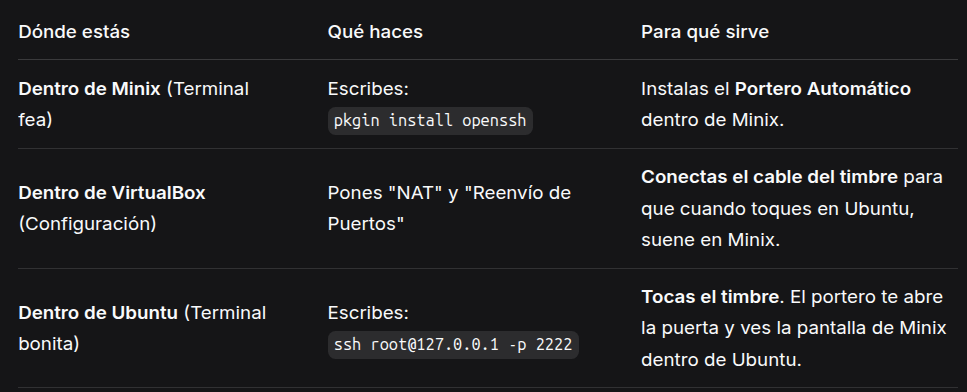
\includegraphics[width=\linewidth]{Deepseek_SSH.png}
        \caption*{Consulta sobre acceso SSH}
    \end{minipage}\hfill
    \begin{minipage}[t]{0.3\textwidth}
        \centering
        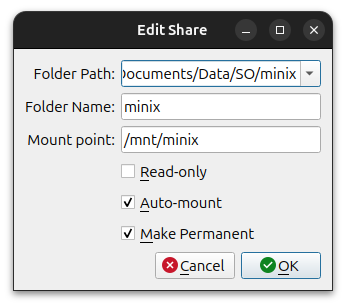
\includegraphics[width=\linewidth]{SF_Config.png}
        \caption*{Configuración de Carpeta Compartida}
    \end{minipage}

    \vspace{0.5em}

    \begin{minipage}{0.62\textwidth}
        \centering
        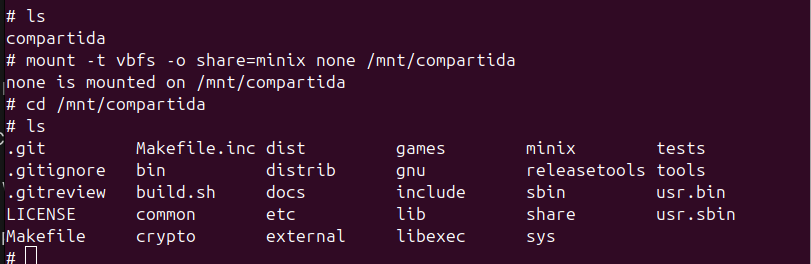
\includegraphics[width=\linewidth]{SF_Mounted.png}
        \caption*{Carpeta Compartida montada en MINIX}
    \end{minipage}
\end{figure}


% ============================================================

\end{document}